\documentclass[12pt]{evalua}
\grado{3$^\circ$ de Secundaria}
\cicloescolar{2022-2023}
\materia{Matemáticas 3}
\guide{2}
\title{Examen de la Unidad}
\aprendizajes{
    \begin{itemize}[leftmargin=*,label=\small\color{colorrds}\faIcon{user-graduate}
        ]
        \item Determina y usa la jerarquía de operaciones y los paréntesis en
              operaciones con números naturales, enteros y
              decimales (para multiplicación y división, sólo números
              positivos).
        \item Calcula valores faltantes en problemas de proporcionalidad
              directa,
              con constante natural, fracción o decimal (incluyendo tablas de
              variación).
    \end{itemize}
}

\author{Prof.: Julio César Melchor Pinto}
\begin{document}
%\printanswers
% {\small
% \begin{multicols}{2}
%     \include*{../blocks/block003}
%     \include*{../blocks/block001}
%     \include*{../blocks/block000}
%     \include*{../blocks/block002}
%     \include*{../blocks/block004}
% \end{multicols}
% % \include*{../blocks/block005}
% % \include*{../blocks/block006}
% }
\begin{questions}
    \question Encuentra el resultado de las siguientes operaciones:

    \begin{multicols}{2}
        \begin{parts}
            \part[5] $\dfrac{3}{7}\times\dfrac{3}{8}=$\\[1em]
            \part[5] $\dfrac{2}{4}\div\dfrac{3}{8}=$\\[1em]
            \part[5] $\dfrac{4}{6}\times\dfrac{5}{8}=$\\[1em]
            \part[5] $\dfrac{1}{3}\div 4=$\\[1em]
            \part[5] $5\times\dfrac{3}{5}=$\\[1em]
            \part[5] $\dfrac{3}{4}\div\dfrac{2}{4}=$\\[1em]
            \part[5] $\dfrac{5}{12}\times\dfrac{6}{8}=$\\[1em]
            \part[5] $7\div\dfrac{4}{9}=$\\[1em]
            \part[5] $\dfrac{11}{12}\times\dfrac{5}{4}=$\\[1em]
        \end{parts}
    \end{multicols}

    \newpage

    \question Obten el resultado de las siguientes operaciones tomando en cuenta la \textbf{jerarquía de operaciones}.

    \begin{multicols}{2}
        \begin{parts}
            \part[5] $3\times 6+5\times\left(10-3\right)^3=$
            \begin{solutionbox}{3cm}
            \end{solutionbox}

            \part[5] $36\div 8+7\times\left(17-2\right)^2=$
            \begin{solutionbox}{3cm}
            \end{solutionbox}

            \part[5] $7+6^2+5-9^3-2=$
            \begin{solutionbox}{3cm}
            \end{solutionbox}

            \part[5] $4\div 2 +8 \div 4 +3=$
            \begin{solutionbox}{3cm}
            \end{solutionbox}

            \part[5] $8\div 2 -\left(2+1\right)\times 2=$
            \begin{solutionbox}{3cm}
            \end{solutionbox}

            \part[5] $4^2\left(2+3\right)- 2\left(2+1\right)=$
            \begin{solutionbox}{3cm}
            \end{solutionbox}
        \end{parts}
        % \end{minipage}

    \end{multicols}

    \newpage

    \question La gráfica de la Figura \ref{fig:escuela_pie} muestra la composición de una escuela de 3 200 personas.

    \begin{figure}[H]
        \centering
        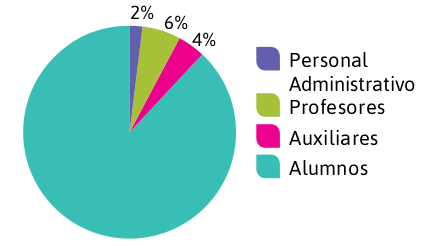
\includegraphics[width=.5\linewidth]{escuela_pie.png}
        \captionof{figure}{Gráfico circular sobre la distribución de los roles en una escuela (en porcentaje).}
        \label{fig:escuela_pie}
    \end{figure}
    % \begin{minipage}{.45\textwidth}

    % \end{minipage}\hfill
    % \begin{minipage}{.45\textwidth}
    \begin{parts}
        \part[5] ¿Cuántas personas trabajan en la administración?
        \begin{solutionbox}{2cm}
        \end{solutionbox}

        \part[5] ¿Cuántos profesores hay en esa escuela?

        \begin{solutionbox}{2cm}
            Los profesores son el 6\% de 3200, entonces:
            \[\dfrac{6}{100}\times 3200=0.06\times 3200=192\]
        \end{solutionbox}

        \part[5] ¿Cuántas personas son auxiliares?

        \begin{solutionbox}{2cm}
        \end{solutionbox}

        \part[5] ¿Cuál es el porcentaje de alumnos?

        \begin{solutionbox}{2cm}
            El porcentaje de alumnos es::
            \[100\%-2\%-6\%-4\%=88\%\]
        \end{solutionbox}

        \part[5] ¿Cuántos alumnos tiene la escuela?
        \begin{solutionbox}{2cm}
        \end{solutionbox}
    \end{parts}
\end{questions}
\end{document}